\subsection{Explicación del algoritmo.}

\vspace*{0.3cm}

Nuestra heuristica golosa elige, para cada nodo, el color que menos apariciones tenga en sus vecinos, asi genera menos conflictos locales. Aunque esto puede ocacionar más conflictos a nivel global, ya que los vecinos de mis vecinos pueden llegar a generar conflictos que se podrían evitar.
Por esto los grafos que mas conflictos generan son los arboles con muchas ramas, ya que la intersección entre los vecinos de un nodo y los vecinos de sus vecinos es el solo los vecinos del nodo.
Para dar una explicacion más detallada del algoritmo veamos el pseudocodigo.

\textbf{pseudocodigo} %\newline 

\begin{codebox}
\Procname{$\proc{hueristica golosa}(Nodo[] \ grafo)	$}
	\li \For $i \gets 0$ \To $size(grafo)$ \Do
	\li		int $cantMinConflictos, cantMinConflictosPos$ = $99999$
	\li 		int[] $colPosibles$ = colores($grafo[i]$)
	\li 		int $colorFinal$ = colores($grafo[i]$)$[0]$
	\li		int $cantVecMismoColor $ = $0$	
	\li		\For $j \gets 0$ \To size($colPosibles$) \Do
	\li	 		int $color$ = $colPosibles[j]$
	\li	 		$cantVecMismoColor$ = $0$
	\li 			\For $k \gets 0$ \To size(sucesores($grafo[i]$)) \Do
	\li 				Nodo $sucesor$ = sucesores($grafo[i]$)$[k]$	
	\li				\If tieneColor($sucesor$) y color($sucesor$) == $color$
	\li					\Then $cantVecMismoColor++$
					\End
				\End
	\li			\If menor($cantVecMismoColor$, $cantMinConflictos$)
	\li				\Then $cantMinConflictos$ = $cantVecMismoColor$
	\li 					$colorFinal$ = $color$
	\li 					$cantMinConflictosPos$ = $0$
	\li 					\For $k \gets 0$ \To size(sucesores($grafo[i]$)) \Do
	\li 						Nodo $sucesor$ = sucesores($grafo[i]$)$[k]$	
	\li						\If !tieneColor($sucesor$) y pertenece($color$, colores($sucesor$))
	\li							\Then $cantMinConflictosPos++$
							\End
						\End
	\li 					\Else 
	\li						\If $cantVecMismoColor$ == $cantMinConflictos$
	\li							\Then int $cantConflictosPosColor$ = $0$
	\li 								\For $k \gets 0$ \To size(sucesores($grafo[i]$)) \Do
	\li 									Nodo $sucesor$ = sucesores($grafo[i]$)$[k]$	
	\li 									\If !tieneColor($sucesor$) y pertenece($color$, colores($sucesor$))
	\li										\Then $cantConflictosPosColor++$
										\End
									\End
	\li								\If menor($cantConflictosPosColor$,$cantMinConflictosPos$)
	\li									\Then $cantMinConflictosPos$ = $cantConflictosPosColor$
	\li 										$colorFinal$ = $color$
									\End
							\End
						\End
				\End
	\li 		color($grafo[i]$) = $color$
			\End
	

\end{codebox}

Nuestro algoritmo para definir los colores recorre todos los nodos y para cada uno de ellos recorre todos sus posibles colores.
Para cada color lo primero que se fija es cuantos vecinos tienen asignado este color, va a ir agarrando el color que menos vecinos de su color tenga. Cuando esto resulte un empate vas a revisar cuantas veces aparece en los posibles colores de sus vecinos, quedandose con el que menos apariciones tenga. Con esto el nodo termina quedandose con el color que menos aparezca en sus vecinos.

%\begin{figure}[htb]
%  \begin{center}
%      \includegraphics[scale=0.25]{imagenes/ejemplo.jpg}
%  \end{center}
%  \caption{ejemplo}
%\end{figure}


\newpage
\subsection{Análisis de complejidad.}

\vspace*{0.3cm}

La complejidad de nuestra heuristaca es O($n^{2}*c^{2}$). La demostración este en la sección 7.4, donde se encuentra el codigo.


\subsection{Experimentación y gráficos.}

\vspace*{0.3cm}

\subsubsection{Test 1}

\vspace*{0.3cm}

\begin{figure}[H]
  \begin{center}
      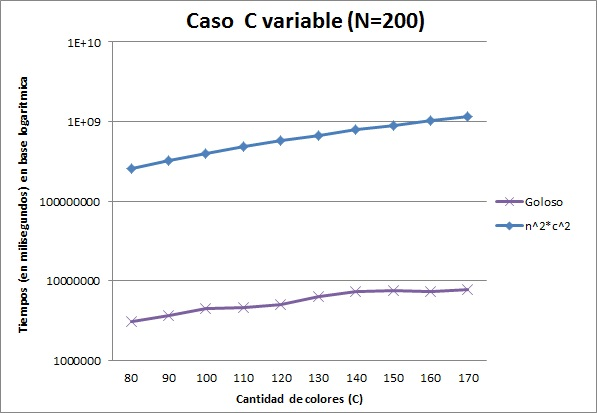
\includegraphics[scale=0.75]{../Ejercicio3CVariable.jpg}
  \end{center}
  \caption{Caso C Variable}
\end{figure}

En este primer gráfico podemos observar que como los nodos, en general,no tienen todos los colores, la variable c no tiene tanta influecia en la complejidad del grafo. Por esto la pendiente de las curvas es poco empinada

\subsubsection{Test 2}

\vspace*{0.3cm}

\begin{figure}[H]
  \begin{center}
      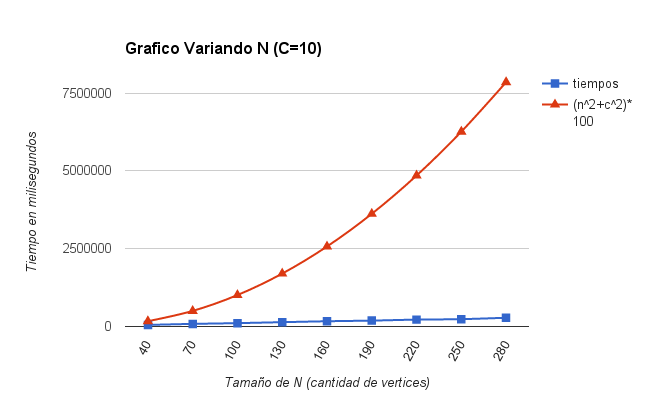
\includegraphics[scale=0.75]{../Ejercicio3VariandoN.png}
  \end{center}
  \caption{Caso N Variable}
\end{figure}

En este grafico podes ver con n es la variable de mayor influencia en la complejidad, ya que al aumentar empieza a aumentar rapidamente la complejidad. Tambíen podemos ver como nuestro algoritmo nunca supera el orden calculado


\subsubsection{Test 3}

\vspace*{0.3cm}

\begin{figure}[H]
  \begin{center}
      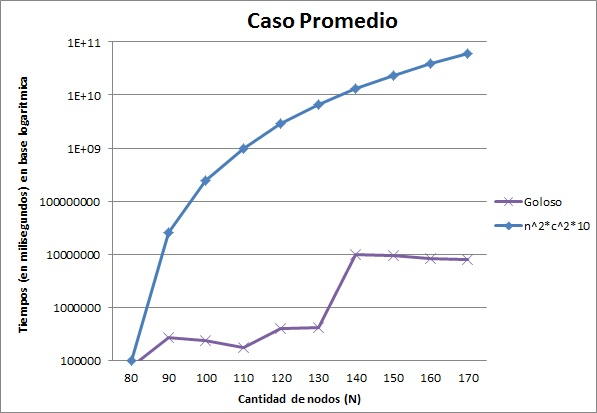
\includegraphics[scale=0.75]{../Ejercicio3Promedio.jpg}
  \end{center}
  \caption{Caso Promedio}
\end{figure}

En este ultimo gráfico podemos corroborar como nuestro algoritmo se mantiene por debajo de la cota propuesta, cabe aclarar que los grafos para esta experimentaci\'on tienen todos sus parametros con randoms, a excepci\'on de n.

\subsubsection{Test 4}

\vspace*{0.3cm}
Ahora miraremos la cantidad de conflictos

\begin{figure}[H]
  \begin{center}
      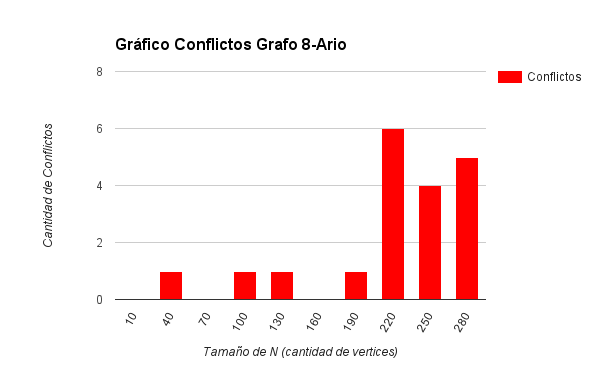
\includegraphics[scale=0.75]{../Ejercicio3Conflictos8-Ario.png}
  \end{center}
  \caption{Grafo 8-Ario}
\end{figure}

Como dijimos antes los grafos que generarian más conflictos son los \'arboles que tienen muchos muchas ramas, es decir los m-arios. En este gr\'afico se puede notar que las primeras instancias tienen menos conflictos, esto se debe a que la altura del \'arbol es demasiado chica y no hay vecinos de vecinos, que como dijimos, son los conflictos que m\'as se pueden dar en nuestra heuristica golosa.
